% This document is used for Daya Bay MACRO PMT pressure test report


\documentclass{beamer}
\usepackage{graphicx}

\newcommand{\tabincell}[2]{\begin{tabular}{@{}#1@{}}#2\end{tabular}}

\usepackage{ragged2e}
\justifying

\usepackage{setspace}

\setbeamertemplate{navigation symbols}{}
\setbeamertemplate{footline}[page number]
\setbeamertemplate{caption}[numbered]

\usetheme{default}
\logo{
\includegraphics[height=1cm]{Dyb_logo.png}}
\begin{document}
\title{Status of MACRO PMT pressure tests at SAB}
\author{Logan Lebanowski, Shih-Kai Lin}
%\institute{University of Houston}
\date{2010 October 14}

\begin{frame}
\begin{center}
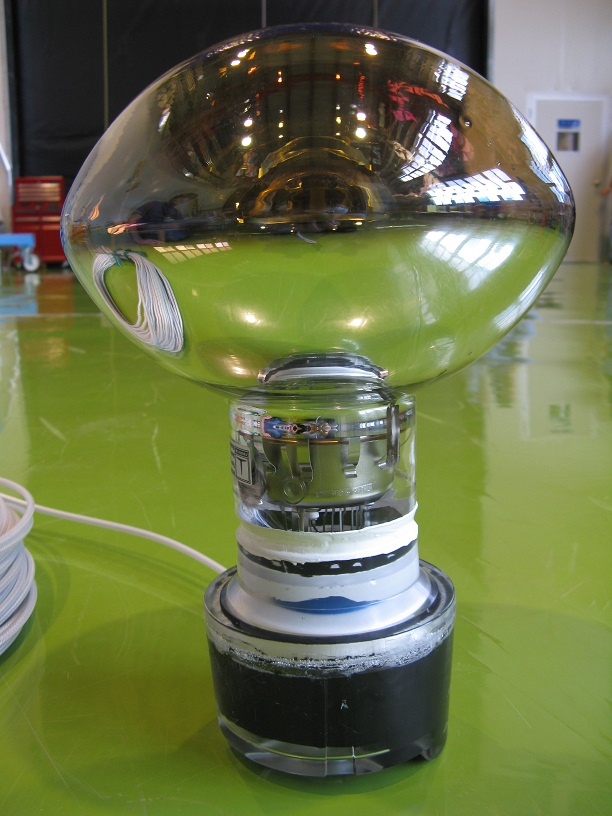
\includegraphics[height=4cm]{IMG_1048.jpg}
\end{center}
\titlepage
\end{frame}


\begin{frame}{overview}
	\begin{itemize}
		\item 150 waterproof MACRO EMI PMT assemblies need to be pressure tested
			at the SAB. They have already passed performance tests at DGUT.
		\item We test about 10 PMTs per week (mid-August to December).
		\item For more information, see
			\textcolor{blue}{\href
			{http://dayabay.ihep.ac.cn/cgi-bin/DocDB/ShowDocument?docid=5373}{doc 5373}}.
	\end{itemize}
		\begin{center}
			\underline{As of October 14, we have passed 70 of 78 tested MACRO PMTs}\\
			\underline{and 1 of 1 tested Hamamatsu PMT.}
		\end{center}
	\begin{center}
		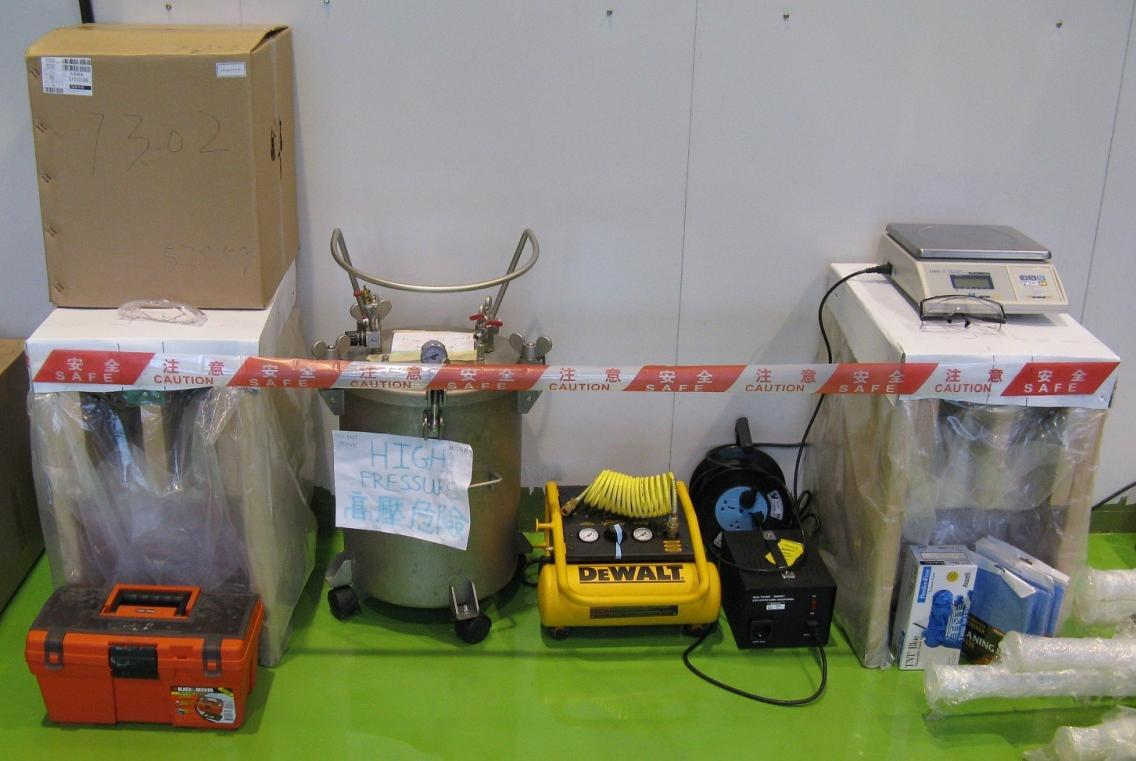
\includegraphics[height=4cm]{test_setup.jpeg}
	\end{center}
\end{frame}


\begin{frame}{pressure test results}
	\begin{center}
		\small
		11 PMTs were tested during the past week (October 7 - October 13).
	\end{center}
\begin{table}
\small
\setstretch{0.4}
\begin{tabular}{|c|c|c|c|c|}
%\setlength{\tabcolsep}{2pt}
	\hline
	SN & mass (g) & pressure (psig) & test time (h:m) & result \\
	\hline
	6289 & 599.0 & 12.0 & 14:50 & PASS$^2$ \\
	\hline
	7315 & 615.5 & 12.1 & 8:38 & PASS$^1$ \\
	\hline
	7431 & 603.5 & 12.0 & 15:01 & PASS$^2$ \\
	\hline
	6400 & 636.5 & 12.1 & 8:25 & PASS$^2$ \\
	\hline
	8618 & 564.0 & 12.0 & 15:49 & PASS$^1$ \\
	\hline
	7487 & 519.0 & 6.0 & 46:45 & PASS$^1$ \\
	\hline
	6623 & 513.0 & 5.8 & 8:22 & PASS$^1$ \\
	\hline
	7508 & 527.5 & 6.1 & 16:09 & PASS$^1$ \\
	\hline
	7492 & 516.0 & 6.1 & 6:44 & PASS$^1$ \\
	\hline
	\tabincell{c}{Hamamatsu$^\dagger$\\WSD2598} & 4631.0$^\ddag$ & 14.2 & 15:23 & PASS$^1$ \\
	\hline
\end{tabular}
%\caption {pressure test result: For PASS/FAIL reasons, please see the table in the next slide.}
\end{table}
	\setstretch{0.1}
	\scriptsize
	$^\dagger$ This is the first water-proof Hamamatsu PMT tested. The PMT holder in the water
	tank held the Hamamatsu PMT well. \\
	$^\ddag$ Weight of PMT, base and cable as a whole.
%\begin{itemize}
%	\item For PASS/FAIL reasons, please see the table in the next slide.
%\end{itemize}
	\setlength{\tabcolsep}{2pt}
	\scriptsize
	\begin{table}
		\begin{tabular}{|c|p{3.5in}|}
		\hline
		1 & Cable dry. No leaks or cracks. \\
		\hline
		2 & 1+Some water penetrated the mastic tape seal of the cable strain relief plug,
			but did not penetrate the UW cable plug. \\
		\hline
%		3 & Cable sealing tube still had some water. The way the cable was repaired didn't
%		work well.\\
%		\hline
		\end{tabular}
	%\caption{PASS/FAIL reasons}
	\end{table}
\end{frame}


\begin{frame}{signal test results}
	\setstretch{0.3}
	\small The operational capability of a PMT is verified after pressure testing:\\
	{\scriptsize The PMT is placed in a dark box, connected to a single channel decoupler box,
	and set to its 2E7 gain voltage, as recorded in the DGUT data. After tens of minutes,
	the count rate, rise time, and pulse height are recorded. We use a threshold of 3.00 
	mV, which is roughly 1/4 pe.
	}

	\setstretch{1}
	\setlength{\tabcolsep}{2pt}
	\small
	\begin{center}
	\begin{tabular}{|l|p{1.2cm}|p{1.9cm}|p{1.5cm}|p{1.7cm}|}
		\hline
		\textbf{SN}&\textbf{Rate (kHz)}&\textbf{DGUT rate (kHz)}&\textbf{Rise time (ns)}&
		\textbf{DGUT rise time (ns)}\\
		\hline
		\hline
%		8727&9.0&0.63&4.1&6.2\\
		8819&4.0&1.08&4.6&4.8\\
		6380&7.0&3.47&4.9&4.2\\
		7925&2.4&0.85&5.9&6.5\\
		7525&7.0&0.40&4.7&7.6\\
		6796&5.2&3.38&4.9&5.1\\
		6289&2.2&0.45&5.0&5.2\\
		7315&2.0&0.64&5.7&6.0\\
		7431&1.0&0.95&4.8&8.7\\
		\hline
	\end{tabular}
		\begin{itemize}
			\item Rates are all below 10 kHz.
		\end{itemize}
	\end{center}
\end{frame}


\end{document}

